% Template LaTeX document for CSSR4A Deliverables
% Adapted from documents prepared by EPFL for the RobotCub project
% and subsequently by the University of Skövde for the DREAM project
%
% DV 28/06/2023

\documentclass{CSSRforAfrica}

\usepackage[titletoc,title]{appendix}
\usepackage[colorlinks, urlcolor=blue, linkcolor=black, citecolor=black]{hyperref}
\usepackage{latexsym}
\usepackage{comment}
\usepackage{multirow}
\usepackage{subcaption}
\usepackage[breakable,skins,most]{tcolorbox} % Consolidated tcolorbox options
\usepackage{tabularx,colortbl}
\usepackage[tikz]{bclogo} % for boxes
\usepackage{ragged2e}
\usepackage{dirtree}
\usepackage{listings}
\usepackage{textcomp}
\usepackage{natbib}
\usepackage{url}
\usepackage{graphicx}
\usepackage{array}
\usepackage{longtable}

\lstset{upquote=true}
\renewcommand{\DTstyle}{\footnotesize\sffamily}

%%% for listing ; added by Pam %%%%%%%%%%%%%%%%%%%%%%%%%%%%%%
\captionsetup[figure]{format=hang}
\definecolor{codegreen}{rgb}{0,0.6,0}
\definecolor{greenyellow}{rgb}{0.8, 0.7, 0.10}
\definecolor{backcolour}{rgb}{0.95,0.95,0.95} 

\lstdefinestyle{withoutNumbering}{
    backgroundcolor=\color{backcolour},   
    commentstyle=\color{codegreen},
    keywordstyle=\color{magenta},
    stringstyle=\color{codepurple},
    basicstyle=\ttfamily\small,
    breakatwhitespace=false,         
    breaklines=true,                 
    captionpos=b,                    
    keepspaces=true,                 
    showspaces=false,                
    showstringspaces=false,
    showtabs=false,                  
    tabsize=2
}
%%%%%%%%%%%%%%%%%%%%%%%%%%%%%%%%%%%%%%%%%%%%%%%%%%%
\newcommand{\blank}{~\\}
\newcommand{\checkbox}{{~~~~~~~\leavevmode \put(-7,-1.5){  \huge $\Box$  }}}

\begin{document}
\input{epsf}

%%
%% SHOULD NOT NEED TO BE CHANGED BEFORE THIS POINT
%% ------------------------------------------------
%%

\deliverable{D5.1}                         
\title{D5.1 Actuator Tests}    

\leadpartner{Carnegie Mellon University Africa} % REPLACE with partner name: Carnegie Mellon University Africa or The University of the Witwatersrand
\partner{}                                      

\revision{1.1}    
\deliverabledate{1/10/2023}    
\submissiondate{26/03/2024}   
\revisiondate{30/05/2025}                
\disseminationlevel{PU}
\responsible{Yohannes Haile}       


%%
%% Create the title page
%%

\maketitle

\section*{Executive Summary}
%==============================================================
Deliverable D5.1 is designed to establish a comprehensive suite of unit tests ensuring the accurate 
and reliable functioning of the actuators. To achieve this, the test will consist of a series of tests 
for the actuators namely head, arms, hands, legs, and wheels. The test will be conducted on both the physical robot 
and the simulator. The central elements of this deliverable comprise the creation of a ROS node named \texttt{actuatorTest},
the generation of a detailed report outlining the developmental procedures, refinement of requirements, and 
explicit definition of functional characteristics. 

Additionally, a user manual will be provided to guide users through the construction and launch of the module. The interface 
design will cover input, output, and control data, while also specifying appropriate data structures. All coding activities 
will strictly adhere to established software engineering standards as set out in Deliverable D3.2. 
\label{executive_summary}

%\graphicspath{{./figs/}}
\pagebreak
\tableofcontents

\newpage

\pagebreak

\section{Introduction}
This document examines the actuator functionality within the Pepper robot, highlighting the pivotal role these components 
play in facilitating its physical interactions. Figure \ref{fig:Pepper_actuator} showcases the distribution of 20 joint 
actuators across Pepper—spanning the head, arms, hands, and wheels—enabling a broad spectrum of movements and behaviors.

The actuators embedded in Pepper's head enable in executing turn and nod motions, thereby fostering engaging interactions 
through nuanced head movements. The arm, and hand actuators empower Pepper with the capability to mimic human gestures, 
significantly enhancing its non verbal communicative and interactive potential. The actuators in the hands further 
permit the opening and closing motions. Such functionality is vital for projects emphasizing non-verbal communication 
through various gestures and movements.

Moreover, the inclusion of actuators in the torso and hips extends Pepper's mobility, allowing it to perform bends and twists. 
This flexibility is crucial for adapting Pepper's movements to reflect various cultural norms of body language, thereby 
augmenting its ability to interact in a culturally sensitive manner. 

The outcomes of the Actuator Test (Deliverable 5.1) are crucial for informing the development of the \texttt{Animate 
Behavior Subsystem} (Deliverable 5.2) by establishing an essential link between the evaluation of actuator performance and 
the enhancement of the Pepper robot's interactive behaviors. 

\begin{figure}[!hbpt]
\centering
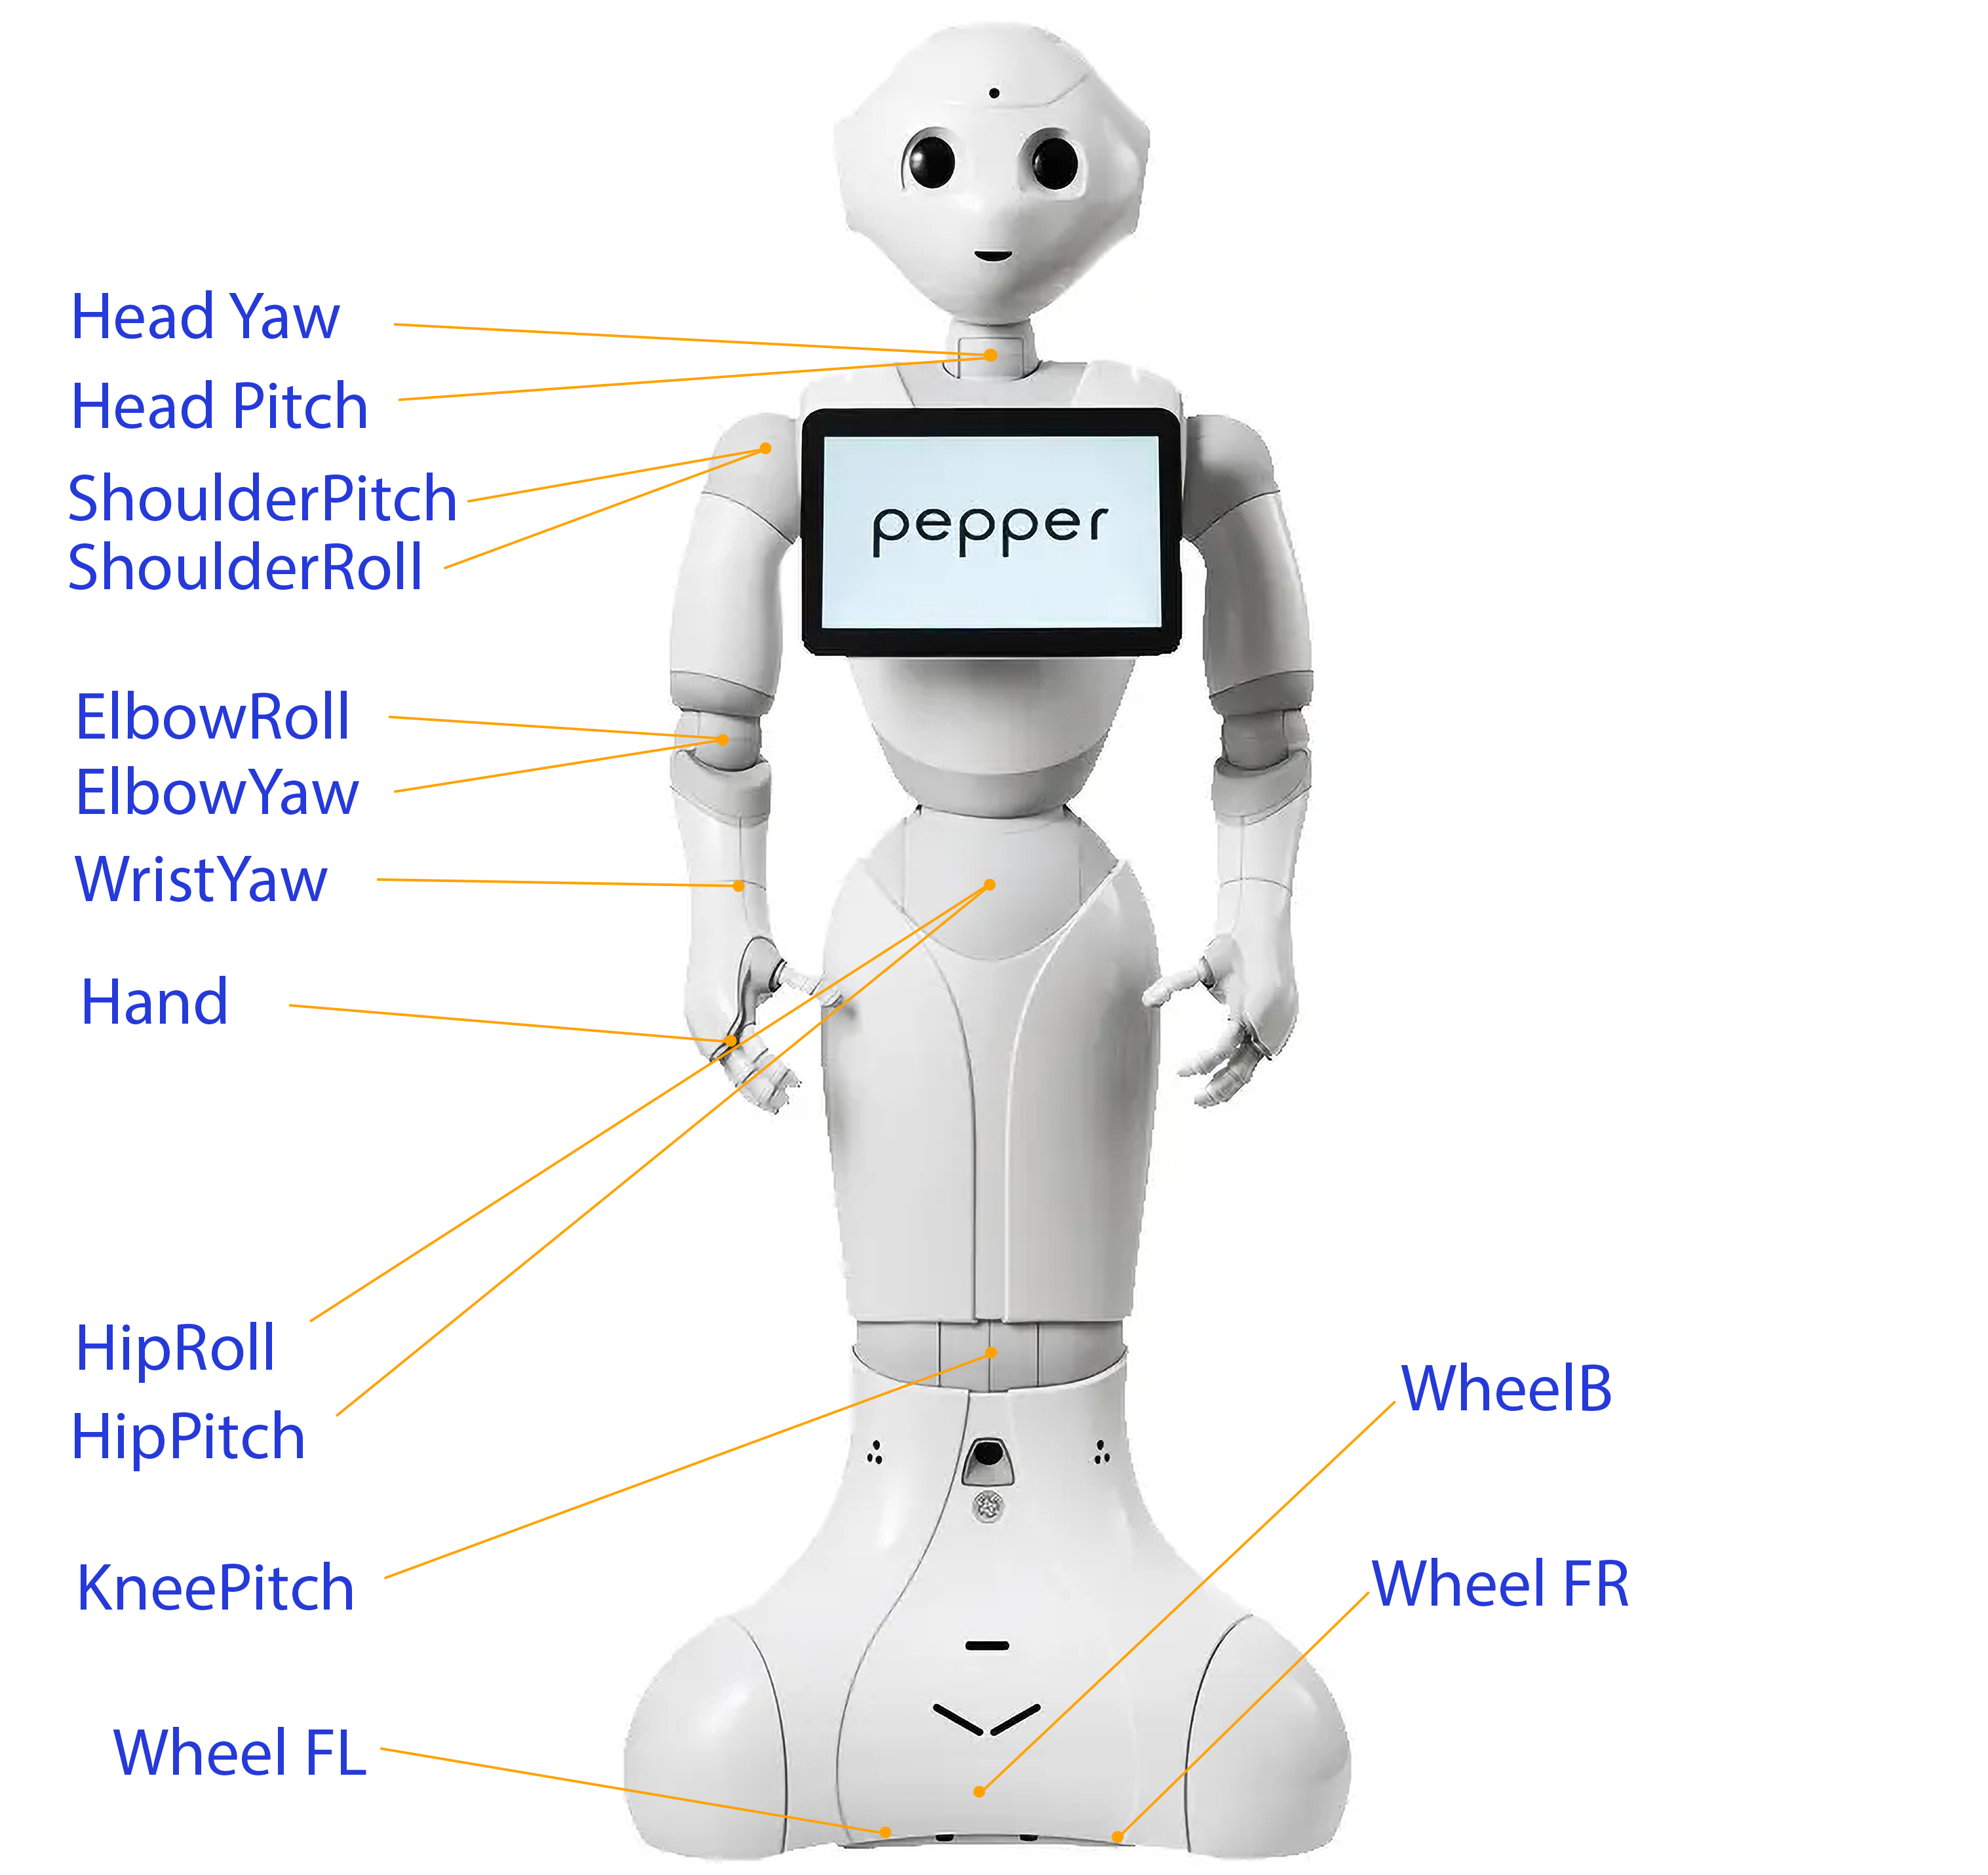
\includegraphics[scale=0.115]{images/Pepper_actuator.png}
\caption{Pepper robot actuators}
\label{fig:Pepper_actuator}
\end{figure}


This deliverable consists of a comprehensive report divided into distinct sections that detail the software development lifecycle. These 
sections encompass the definition of requirements, aligning functional necessities with project goals, module specifications detailing the 
testing methodologies for joint and wheel actuators, and the design of interfaces, specifying data exchange via the ROS middleware and file inputs.

Additionally, the deliverable outlines the module's operation, governed by configurations detailed in \texttt{actuatorTestConfiguration.ini}, and 
delineates the structure for message data handling. Furthermore, a user manual for effective deployment and configuration, ensuring a smooth integration 
into the testing framework for both physical and simulated Pepper robot platforms. The coding section provides the implemented program code, adhering 
to standards specified in Deliverable D3.2. 

\newpage

\section{Requirements Definition}
The actuator test provides a systematic process aimed at understanding and documenting the functional and non-functional
needs that the module must fulfill. This deliverable is important in identifying the specific user expectations, 
ensuring that the module will be capable of performing the precise actuator tests in various scenarios, including different
operations and environments (physical robot and simulator). The test encompasses a thorough examination of the intended 
functionality, such as actuator identification, movement control, and the ability to conduct tests in sequence or parallel.

As seen from the diagram in Figure \ref{fig:Pepper_actuator}, the Pepper robot has 20 joint actuators and 3 wheel actuator.
For joint actuators, the module must be able to move each joint to its minimum, maximum, and mid-range positions at specified 
average angular velocities. For wheel actuators, the module should conduct tests at designated positive and negative angular 
and linear velocities.

\subsection*{Misalignment of the Module}
In addition to joint and wheel actuators, the robot features loudspeakers capable of generating speech from text. However, 
this phase does not encompass loudspeaker testing due to the absence of the required rostopic in the NAOqi DCM driver. 
Therefore, loudspeaker evaluation is incorporated into the \texttt{Sensor Test} deliverable.

While the physical robot is equipped with hand actuators, this feature is missing in the simulator. Consequently, hand 
actuator testing is exclusive to the physical robot.

Another noted limitation concerns the robot's performance during parallel actuator testing. The robot struggles with 
simultaneous activation of multiple actuators, particularly affecting performance when wheel actuators are tested. 
This issue necessitates conducting wheel actuator tests sequentially to prevent the delay encountered during parallel 
testing.

\newpage

\section{Module Specifications}

\subsection*{Joint actuator}
To validate the range of motion and control accuracy of each joint actuator by moving it through its minimum, mid-range, 
and maximum positions.

During the initialization phase, an average angular velocity ($\dot{\theta}$) is selected for the movement of each actuator. 
In the test execution phase, each joint is moved to its minimum position at the predetermined $\dot{\theta}$, and the 
duration required for this movement ($\Delta t$) is calculated using the formula $\Delta t = \Delta \theta / \dot{\theta}$, 
where $\Delta \theta$ represents the total change in the actuator's angle. This procedure is then systematically repeated 
to position the joint at its mid-range and maximum values. The testing procedure will have the following order:
$\texttt{home position} \rightarrow \texttt{minimum position} \rightarrow \texttt{maximum position} \rightarrow \texttt{mid-range 
position} \rightarrow \texttt{home position}$. In the verification phase, it is crucial to confirm that each 
joint accurately reaches these designated positions.

\subsection*{Wheel actuator}
To assess the wheel actuator's capability to execute controlled rotational and linear movements.

The test procedures initiate with the evaluation of the robot's linear motion capabilities, subsequently moving on to its 
rotational dynamics. In the linear movement test, the robot moves at a specified positive linear velocity, for instance, 
1 m/s, for a pre-determined time. This procedure is then mirrored using a negative linear velocity, such 
as -1 m/s, to assess the robot's proficiency in reverse movements. Following the linear evaluation, the rotational movement test 
is conducted. Here, the robot is commanded to rotate at a chosen positive angular velocity, such as 90°/s, for a fixed interval. 
The fidelity of this rotation is thoroughly inspected, with any deviations from expected behavior being noted. This 
is again performed with a negative angular velocity, for example, -90°/s, to confirm the robot's rotational consistency in both 
directions and to log any variations observed.

\newpage

\section{Interface Design}
\subsection*{File Organization}
The source code for conducting actuator tests is structured into two primary components: \\
\texttt{actuatorTestApplication} and \texttt{actuatorTestImplementation}. The actuatorTestImplementation 
component encapsulates all the essential functionality required for executing comprehensive actuator tests. 
This includes all of the tests for the actuators that consist of the head, arms, hands, legs, and wheels.
Similar to the sensor test, the actuator test is also equipped with the functionality to process various files
critical for the testing process, such as configuration files, input files, and topic files.

On the other hand, the actuatorTestApplication invokes those functions for the testing process. It is tasked with the
execution of functions defined within the actuatorTestImplementation, effectively managing the actuator test operations.\\

Here is the file structure of the pepper interface tests package:

\vspace*{0.5em}

\renewcommand*\DTstyle{\ttfamily}
\dirtree{%
.1 pepper\_interface\_tests.
.2 config.
.3 actuatorTestConfiguration.ini.
.3 actuatorTestInput.ini.
.3 sensorTestInput.ini.
.3 sensorTestConfiguration.ini.
.2 data.
.3 pepperTopics.dat.
.3 sensorTestOutput.dat.
.3 simulatorTopics.dat.
.2 include.
.3 pepper\_interface\_tests.
.4 actuatorTestInterface.h.
.4 sensorTestInterface.h.
.2 launch.
.3 actuatorTestLaunchRobot.launch.
.3 sensorTestLaunchRobot.launch.
.3 interfaceTestLaunchSimulator.launch.
.2 src.
.3 actuatorTestApplication.cpp.
.3 actuatorTestImplementation.cpp.
.3 sensorTestApplication.cpp.
.3 sensorTestImplementation.cpp.
.2 README.md.
.2 CMakeLists.txt.
.2 package.xml.
}

\newpage

\subsection*{Configuration File}
The operation of the actuatorTest node is determined by the contents of the configuration file that contains a 
list of key-value pairs as shown below.

The configuration file is named \texttt{actuatorTestConfiguration.ini}

% Table of 3 x 4 with the following headers: Key, Value, Description
\begin{longtable}[c]{|l|l|p{7cm}|}
    \caption{Configuration file for the actuator test.} \label{tab:config_file}\\
    \hline
    \rowcolor{gray!30}
    \small{\textbf{Key}} & \small{\textbf{Value}} & \small{\textbf{Description}} \\ \hline
    \endhead % header for subsequent pages
    
    \small{\texttt{platform}} & \small{\texttt{simulator}} or \texttt{robot} & \small{Specifies the platform to be tested. The platform can be set to either \texttt{simulator} or \texttt{robot}.} \\ \hline
    \small{\texttt{robotTopics}} & \small{\texttt{robotTopics.dat}} & \small{Specifies the name of the robot topics file. The robot topics file contains the list of topics for the robot.} \\ \hline
    \small{\texttt{simulatorTopics}} & \small{\texttt{simulatorTopics.dat}} & \small{Specifies the name to the simulator topics file. The simulator topics file contains the list of topics for the simulator.} \\ \hline
    \small{\texttt{mode}} & \small{\texttt{parallel}} or \texttt{sequential} & \small{Specifies the mode of the test. The mode can be either \texttt{parallel} or \texttt{sequential}. The parallel mode runs all the tests in parallel. The sequential mode runs all the tests sequentially.} \\ \hline
\end{longtable}

\subsection*{Input File}
The input file is used to specify which actuators to test by using the actuator name as the key and \texttt{True} or \texttt{False} as the value.
The actuator name must be the same as the actuator name in the topics file.

The input file is named \texttt{actuatorTestInput.ini}

\subsection*{Output Data File}
There is no output data file for the actuator test. The result of the test is printed on the terminal.

\subsection*{Topics File}
For the test, a selected list of the topics for the robot and simulator is stored in the topics file. The topic files are written in the .dat file format.
The data file is written in key-value pairs where the key is the actuator name and the value is the topic

The topics file for the robot is named \texttt{robotTopics.dat} and the topics file for the simulator is named \texttt{simulatorTopics.dat}.

\subsubsection*{Topics Subscribed}
There is no topics subscribed by the actuatorTest node.

\newpage

\subsubsection*{Topics Published}
The actuatorTest node publishes the following topics

\begin{longtable}[c]{|l|l|l|}
    \caption{Topics Published by the actuatorTest node.} \label{tab:Published_topics} \\
    \hline
    \rowcolor{gray!30}
    \footnotesize{\textbf{Topic}} & \footnotesize{\textbf{Actuator}} & \footnotesize{\textbf{Platform}} \\ \hline
    \endhead % header for subsequent pages
    
    \footnotesize{\texttt{/pepper\_dcm/Head\_controller/follow\_joint\_trajectory}} & \footnotesize{\texttt{Head}} & \footnotesize{\texttt{robot}} \\ \hline
    \footnotesize{\texttt{/pepper\_dcm/LeftArm\_controller/follow\_joint\_trajectory}} & \footnotesize{\texttt{Left Arm}} & \footnotesize{\texttt{robot}} \\ \hline
    \footnotesize{\texttt{/pepper\_dcm/RightArm\_controller/follow\_joint\_trajectory}} & \footnotesize{\texttt{Right Arm}} & \footnotesize{\texttt{robot}} \\ \hline
    \footnotesize{\texttt{/pepper\_dcm/LeftHand\_controller/follow\_joint\_trajectory}} & \footnotesize{\texttt{Left Hand}} & \footnotesize{\texttt{robot}} \\ \hline
    \footnotesize{\texttt{/pepper\_dcm/RightHand\_controller/follow\_joint\_trajectory}} & \footnotesize{\texttt{Right Hand}} & \footnotesize{\texttt{robot}} \\ \hline
    \footnotesize{\texttt{/pepper\_dcm/Pelvis\_controller/follow\_joint\_trajectory}} & \footnotesize{\texttt{Leg}} & \footnotesize{\texttt{robot}} \\ \hline
    \footnotesize{\texttt{/cmd\_vel}} & \footnotesize{\texttt{Wheels}} & \footnotesize{\texttt{robot}} \\ \hline
    \footnotesize{\texttt{/pepper/Head\_controller/follow\_joint\_trajectory}} & \footnotesize{\texttt{Head}} & \footnotesize{\texttt{simulator}} \\ \hline
    \footnotesize{\texttt{/pepper/LeftArm\_controller/follow\_joint\_trajectory}} & \footnotesize{\texttt{Left Arm}} & \footnotesize{\texttt{simulator}} \\ \hline
    \footnotesize{\texttt{/pepper/RightArm\_controller/follow\_joint\_trajectory}} & \footnotesize{\texttt{Right Arm}} & \footnotesize{\texttt{simulator}} \\ \hline
    \footnotesize{\texttt{/pepper/LeftHand\_controller/follow\_joint\_trajectory}} & \footnotesize{\texttt{Left Hand}} & \footnotesize{\texttt{simulator}} \\ \hline
    \footnotesize{\texttt{/pepper/RightHand\_controller/follow\_joint\_trajectory}} & \footnotesize{\texttt{Right Hand}} & \footnotesize{\texttt{simulator}} \\ \hline
    \footnotesize{\texttt{/pepper/Pelvis\_controller/follow\_joint\_trajectory}} & \footnotesize{\texttt{Leg}} & \footnotesize{\texttt{simulator}} \\ \hline
    \footnotesize{\texttt{/pepper/cmd\_vel}} & \footnotesize{\texttt{Wheels}} & \footnotesize{\texttt{simulator}} \\ \hline
\end{longtable}

\subsection*{Launch File}
The \texttt{actuatorTestLaunchRobot.launch} launch file is used to launch the actuator test. It is used for the robot and \texttt{actuatorTestLaunchSimulator.launch} for the simulator.
The robot has launch file has the following parameters:

\begin{itemize}
    \item \texttt{robot\_ip}: specifies the IP address of the robot.
    \item \texttt{roscore\_ip}: specifies the IP address of the roscore.
    \item \texttt{network\_interface}: specifies the network interface name.  
\end{itemize}


A default value is provided for each parameter in the launch file. For the robot ip, the default value 
is \texttt{172.29.111.230} and for the network\_interface, the default value is \texttt{eth0}. The roscore 
ip does not have a default value and must be provided when launching the file.

\newpage

The diagram below shows the data flow of the actuator test. The actuator test node reads the configuration file,
input file, and topics file. The robot or simulator receives the topics and executes the tests. The robot or 
simulator then publishes the results to the actuator test node.

\begin{figure}[!hbpt]
\centering
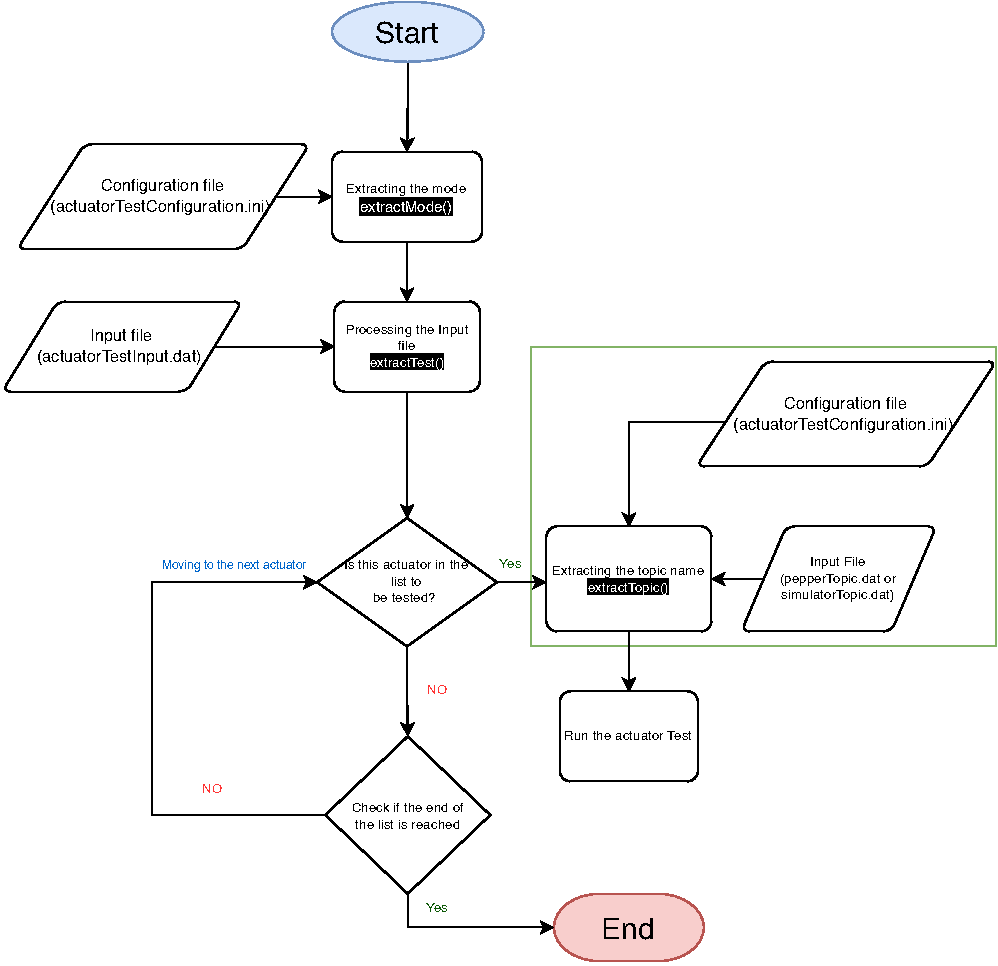
\includegraphics[scale=0.9]{images/Actuator.pdf}
\caption{Data Flow of the Actuator Test}
\label{fig:actuator_test}
\end{figure}


\newpage

\section{Module Design}

For testing the physical robot, the NAOqi DCM (Device Communication Manager) driver is used to control the robot's actuators. 
The driver provides a hardware interface to connect to Alderban's robot Nao, Romeo, and Pepper robots. There are two ways to 
control the robot: DCM commands or ALMotion(default). DCM commands control the robot at a faster frequency but it sometimes 
results in the robot shaking. Hence, the test for the actuator is done using ALMotion. 

The module is designed using to move the joint actuator of  robot to a specified position by defining trajectory goal and sending it 
to a control server via a ROS(Robot Operating System) topic. First, the module initializes a client for interacting 
with ROS actions server. The function is structured attempt to attempt a connection to the server. If the connection 
to the server multiple times before giving up and throwing an error. The function \texttt{ControlClientPtr 
createClient(const std::string\& topicName)} takes in the the topic name and returns actionClient pointer. 

After the client is created, the module commands the robot to move to a specified position by defining a trajectory
goal and sending it to the control server via ROS action client. First, the module will define a goal message for 
a joint trajectory action, which is part of the \texttt{control\_msgs} package. The \texttt{follow\_joint\_trajectory}
action is used to generate a more complex motion control mechanism, often used for executing predefined paths or
trajectories for a set of joints. 

The components of this topic include: 
\begin{itemize}
    \item \texttt{/goal}: used to send a ``FollowJointTrajectoryGoal", which includes a trajectory comprising multiple points (position, 
    velocities, acceleration, and/or efforts for each joint) and the time at which those points should be reached.
    \item \texttt{/cancel}: can cancel a currently executing trajectory.
    \item \texttt{/feedback}: provides real-time feedback about the current state of the trajectory 
    execution. 
    \item \texttt{/result}: provides the outcome of the trajectory execution after completion.
    \item \texttt{/status}: provides status information about the goal, such as if it's active, succeeded, or aborted
\end{itemize} 

The trajectory goal will be send to the action server through the client. The server, presumably a part of a 
motion control system, will interpret this goal and command the robotic arm to move accordingly. The system 
then waits for a fixed duration for the movement to complete before proceeding.\\

The wheel test is done by publishing on the \texttt{cmd\_vel} topic. The \texttt{cmd\_vel} topic is used to control the
robot's wheels. The message type used for the \texttt{cmd\_vel} topic is \texttt{geometry\_msgs/Twist}. The \texttt{Twist}
message type is used to send velocity commands to the robot. The \texttt{Twist} message contains two \texttt{Vector3}
messages, one for linear velocity and one for angular velocity. The \texttt{Vector3} message type is used to send
three-dimensional linear and angular velocity commands.

\pagebreak

\section{Executing the Actuator Tests}
To start the actuator test, the user must first install the necessary software packages as outlined in \href{https://cssr4africa.github.io/deliverables/CSSR4Africa_Deliverable_D3.3.pdf}
{Deliverable D3.3}. Referring to the interface section, the user must set the platform to be tested, and specify which mode to run the test. Then using the key-value pairs, the users must
specify which actuators to test by using the actuator name as the key and \texttt{True} or \texttt{False} as the value. To launch the actuator, the user must run the following command:

\begin{lstlisting}[style=withoutNumbering, language=bash]
# Launch the Actuator Test for the physical robot
roslaunch pepper_interface_tests actuatorTestLaunchRobot.launch \
robot_ip:=<robot_ip> roscore_ip:=<roscore_ip> \
network_interface:=<network_interface>
\end{lstlisting}

\begin{lstlisting}[style=withoutNumbering, language=bash]
# Launch the Actuator Test for the simulator
roslaunch pepper_interface_tests actuatorTestLaunchSimulator.launch
\end{lstlisting}

The above command will launch the actuator test for the robot and simulator respectively. After 
launching the actuators test, the user will run the tests by using the following command:

\begin{lstlisting}[style=withoutNumbering, language=bash]
rosrun pepper_interface_tests actuatorTest
\end{lstlisting}

\begingroup
\tcbset{%
noteshift/.store in=\mynote@shift,
noteshift=0.8cm
}
\begin{tcolorbox}[nobeforeafter,
enhanced,
sharp corners,
toprule=1pt,
bottomrule=1pt,
leftrule=0pt,
rightrule=0pt,
colback=yellow!20,
left skip=\mynote@shift,
right skip=\mynote@shift,
overlay={\node[left] (mynotenode) at ([xshift=-\mynote@shift]frame.west) {\textbf{\textcolor{greenyellow}{Note:}}} ;},]
A noted limitation occurs when operating the robot in parallel mode: the robot's joint actuator cannot function concurrently
while the robot is moving. Specifically, when the robot is executing movement commands via the \texttt{cmd\_vel} topic, the joint actuator
cannot be engaged simultaneously. To prevent any operational conflicts, it is essential to conduct a few test on the joint actuator only when the robot 
remains stationary.
\end{tcolorbox}
\endgroup

Some technical details of the joints will be in the sections below. Refer to the 
\href{http://doc.aldebaran.com/2-5/family/pepper_technical/joints_pep.html}{Pepper Technical Documentation} for more information on the joints.

\subsection{Head Actuator Test}
As shown in Figure \ref{fig: Pepper Head joint} there are two joints in the head of the Pepper robot which are the \texttt{HeadYaw} and \texttt{HeadPitch}.
The head Yaw joint is responsible for the left and right movement of the head while the head pitch joint is responsible for the up and down movement of the head. The test is conducted by moving both joints in the following sequence:
$ \texttt{Home pos} \rightarrow \texttt{Minimum pos} \rightarrow \texttt{Maximum pos} \rightarrow \texttt{Mid-range pos} \rightarrow \texttt{Home pos}$.
The terminal output will show the result of the test. The head joint range is shown in the table \ref{tab:head_joint_range}.

\begin{longtable}[c]{|l|l|l|l|l|l|} 
    \caption{Head Joint Range. \cite{PepperJoints}} \label{tab:head_joint_range}\\
    \hline
    \rowcolor{gray!30}
    \textbf{Joint} & \textbf{Min (°)} & \textbf{Max (°)} & \textbf{Min (rad)} & \textbf{Max (rad)} & \textbf{Home (rad)} \\ \hline
    \endhead % header for subsequent pages
    
    \texttt{HeadYaw} & -119.5 & 119.5 & -2.0857 & 2.0857 & -0.2 \\ \hline
    \texttt{HeadPitch} & -40.5 & 25.5 & -0.7068 & 0.4451 & 0.01 \\ \hline
    
\end{longtable}

\newpage

\begin{figure}[!hbpt]
\centering
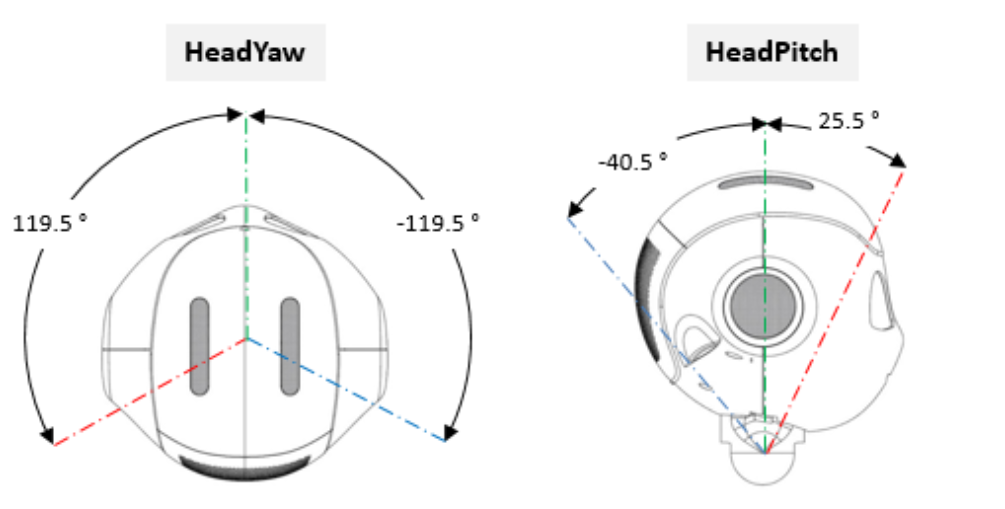
\includegraphics[scale=0.35]{images/Pepper_Head.png}
\caption{Pepper Head Joint \cite{PepperJoints}}
\label{fig: Pepper Head joint}
\end{figure}

The rostopic \texttt{/pepper\_dcm/Head\_controller/follow\_joint\_trajectory} moves the head joint.

Due to the collision with the robot's body, some head joint positions are not reachable. So when specifying the position, the user must be mindful of the limits especially when planning to move the head in a certain trajectory. The table \ref{tab:head_joint_limits} shows the limits of the head joint.

% Table of 3 x 4 with the following headers: HeadYaw (°), HeadPitch - (°), HeadPitch + (°)
\begin{longtable}[c]{|l|l|l|l|} 
    \caption{Head joint limits. \cite{PepperJoints}} \label{tab:head_joint_limits}\\
    \hline
    \rowcolor{gray!30}
    \textbf{HeadYaw (°)} & \textbf{HeadPitch - (°)} & \textbf{HeadPitch + (°)} \\ \hline
    \endhead % header for subsequent pages
    
    -119.5 & -35.0 & 13.5 \\ \hline
    -91.4 & -35.1 & 13.5 \\ \hline
    -61.6 & -35.2 & 20.9 \\ \hline
    -33.33 & -40.5 & 36.5 \\ \hline
    33.33 & -40.5 & 36.5 \\ \hline
    61.6 & -35.2 & 20.9 \\ \hline
    91.4 & -35.1 & 13.5 \\ \hline
    119.5 & -35.0 & 13.5 \\ \hline
\end{longtable}

\subsection{Arm Actuator Test}
\subsubsection*{Left Arm}
The left arm of the Pepper robot is articulated with five distinct joints: \texttt{LShoulderPitch},\\
\texttt{LShoulderRoll}, \texttt{LElbowYaw}, \texttt{LElbowRoll}, and
\texttt{LWristYaw}. These joints are tested sequentially in the listed order to ensure proper functionality and range of motion. The testing involves moving each joint through a specific sequence of positions to verify the joint's operational range and functionality as follows:\\
$ \texttt{Home pos} \rightarrow \texttt{Minimum pos} \rightarrow \texttt{Maximum pos} \rightarrow \texttt{Mid-range pos} \rightarrow \texttt{Home pos}$.

The rostopic \texttt{/pepper\_dcm/LeftArm\_controller/follow\_joint\_trajectory} is used to move the 
left arm joint.

Table \ref{tab:left_arm_joint_range} shows the range of the left arm joint.


\begin{longtable}[c]{|l|l|l|l|l|l|} 
    \caption{Left Arm Joint Range.\cite{PepperJoints}} \label{tab:left_arm_joint_range}\\
    \hline
    \rowcolor{gray!30}
    \textbf{Joint} & \textbf{Min (°)} & \textbf{Max (°)} & \textbf{Min (rad)} & \textbf{Max (rad)}  & \textbf{Home (rad)} \\ \hline
    \endhead % header for subsequent pages
    
    \texttt{LShoulderPitch} & -119.5 & 119.5 & -2.0857 & 2.0857 & 1.7625 \\ \hline
    \texttt{LShoulderRoll} & 0.5 & 89.5 & 0.0087 & 1.5620 & 0.09970 \\ \hline
    \texttt{LElbowYaw} & -119.5 & 119.5 & -2.0857 & 2.0857 & -1.7150 \\ \hline
    \texttt{LElbowRoll} & -89.5 & -0.5 & -1.5620 & -0.0087 &  -0.1334 \\ \hline
    \texttt{LWristYaw} & -104.5 & 104.5 & -1.8239 & 1.8239 & 0.06592 \\ \hline

\end{longtable}

\begin{figure}[!hbpt]
\centering
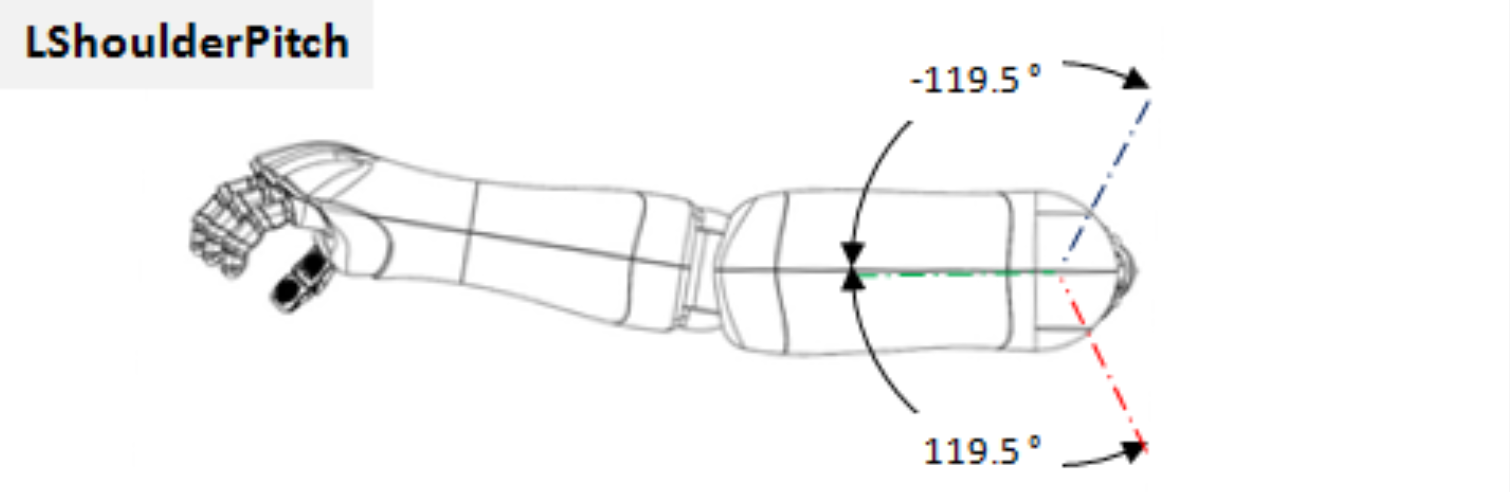
\includegraphics[scale=0.35]{images/LShoulderPitch.png}
\caption{Left Shoulder Pitch Joint \cite{PepperJoints}}
\label{fig: Left Shoulder Pitch joint}
\end{figure}

\begin{figure}[!hbpt]
    \centering
    \begin{minipage}{0.45\textwidth}
        \centering
        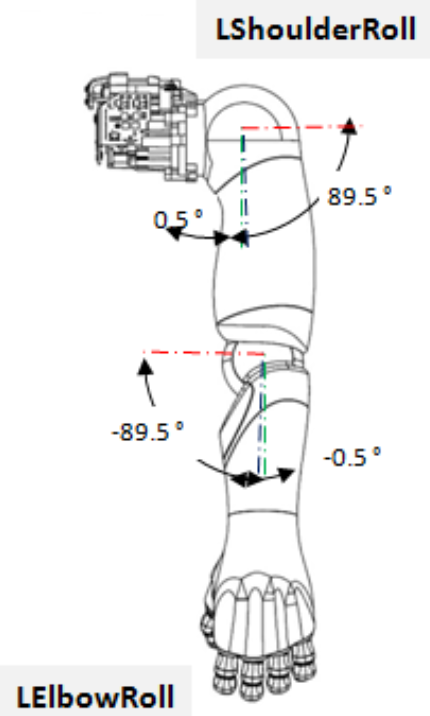
\includegraphics[scale=0.45]{images/LShoulderandLElbowRoll.png}
        \caption{Left Shoulder Roll and Elbow Roll Joint \cite{PepperJoints}}
        \label{fig: Left Shoulder Roll and Elbow Roll joint}
    \end{minipage}\hfill
    \begin{minipage}{0.45\textwidth}
        \centering
        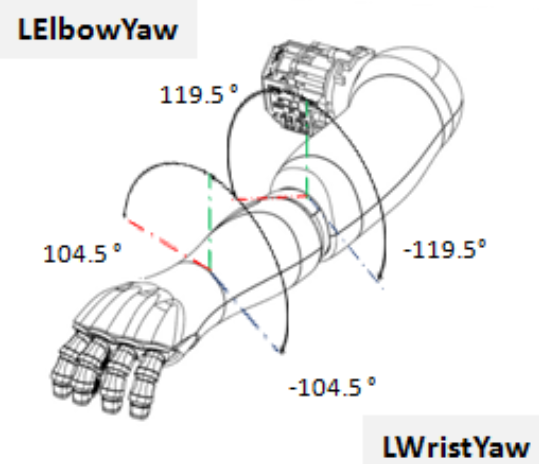
\includegraphics[scale=0.45]{images/LElbowandWristYaw.png}
        \caption{Left Elbow and Wrist Joint \cite{PepperJoints}}
        \label{fig: Left Elbow and Wrist joint}
    \end{minipage}
\end{figure}

\newpage

Due to collision, the LElbowRoll is limited. The table \ref{tab:left_arm_joint_limits} shows the limits of the 
left Elbow Roll joint.

\begin{longtable}[c]{|l|l|l|l|} 
    \caption{Left Arm Joint Limits.\cite{PepperJoints}} \label{tab:left_arm_joint_limits}\\
    \hline
    \rowcolor{gray!30}
    \textbf{LElbowYaw (°)} & \textbf{LElbowRoll Min (°)} & \textbf{LElbowRoll Max (°)} \\ \hline
    \endhead % header for subsequent pages
    
    -119.5 & -78.0 & -0.5 \\ \hline
    -60.0 & -78.0 & -0.5 \\ \hline
    0.0 & -89.5 & -0.5 \\ \hline
    99.5 & -89.5 & -0.5 \\ \hline
    119.5 & -83.0 & -0.5 \\ \hline

\end{longtable}


\subsubsection*{Right Arm}
The right arm of the Pepper robot is articulated with five distinct joints: \texttt{RShoulderPitch},\\ 
\texttt{RShoulderRoll}, \texttt{RElbowYaw}, \texttt{RElbowRoll}, and
\texttt{RWristYaw}. These joints are tested sequentially in the listed order to ensure proper functionality and range of motion. The testing involves moving each joint 
through a specific sequence of positions to verify the joint's operational range and functionality as follows:\\
$ \texttt{Home pos} \rightarrow \texttt{Minimum pos} \rightarrow \texttt{Maximum pos} \rightarrow \texttt{Mid-range pos} \rightarrow \texttt{Home pos}$.

To make the movement symmetrical with the left arm, the \texttt{RShoulderPitch} joint is moved from the maximum position to the minimum position instead of the minimum position to the maximum position. While still having a home position as the starting and ending position. The terminal output will output each phase of the joint movement.

The rostopic \texttt{/pepper\_dcm/RightArm\_controller/follow\_joint\_trajectory} moves the right arm joint.

Table \ref{tab:right_arm_joint_range} shows the range of the right arm joint.

\begin{longtable}[c]{|l|l|l|l|l|l|} 
    \caption{Right Arm Joint Range.\cite{PepperJoints}} \label{tab:right_arm_joint_range}\\
    \hline
    \rowcolor{gray!30}
    \textbf{Joint} & \textbf{Min (°)} & \textbf{Max (°)} & \textbf{Min (rad)} & \textbf{Max (rad)}  & \textbf{Home (rad)} \\ \hline
    \endhead % header for subsequent pages
    
    \texttt{RShoulderPitch} & -119.5 & 119.5 & -2.0857 & 2.0857 & 1.7410 \\ \hline
    \texttt{RShoulderRoll} & -89.5 & -0.5 & -1.5620 & -0.0087 & -0.09664 \\ \hline
    \texttt{RElbowYaw} & -119.5 & 119.5 & -2.0857 & 2.0857 & 1.6981 \\ \hline
    \texttt{RElbowRoll} & 0.5 & 89.5 & 0.0087 & 1.5620 & 0.09664 \\ \hline
    \texttt{RWristYaw} & -104.5 & 104.5 & -1.8239 & 1.8239 & -0.05679 \\ \hline

\end{longtable}

\begin{figure}[!hbpt]
\centering
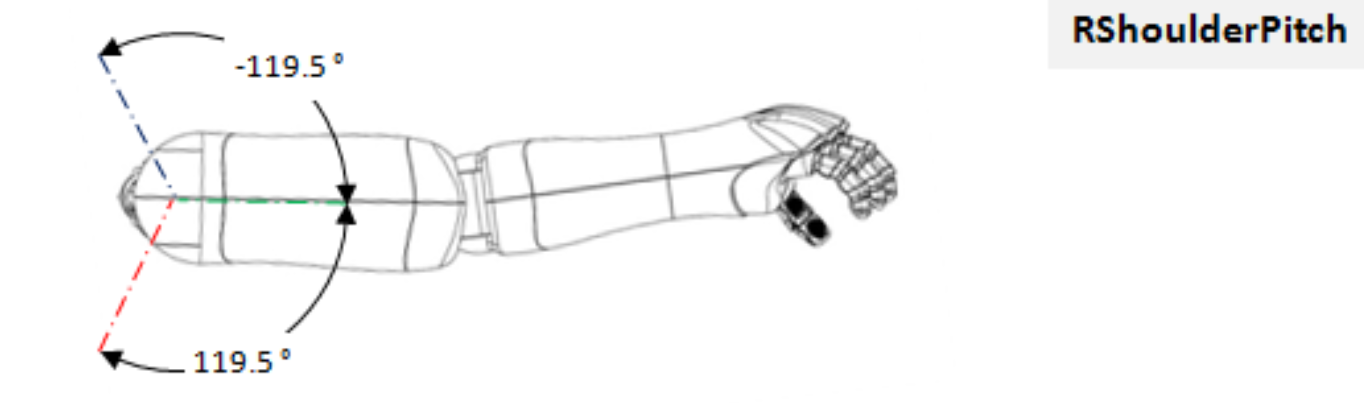
\includegraphics[scale=0.35]{images/RShoulderPitch.png}
\caption{Right Shoulder Pitch Joint \cite{PepperJoints}}
\label{fig: Right Shoulder Pitch joint}
\end{figure}

\newpage

\begin{figure}[!hbpt]
    \centering
    \begin{minipage}{0.45\textwidth}
        \centering
        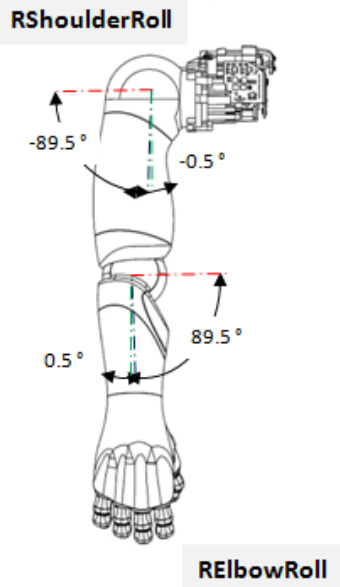
\includegraphics[scale=0.45]{images/RShoulderandElbowRoll.png}
        \caption{Right Shoulder and Elbow Roll Joint \cite{PepperJoints}}
        \label{fig: Right Shoulder and Elbow Roll joint}
    \end{minipage}\hfill
    \begin{minipage}{0.45\textwidth}
        \centering
        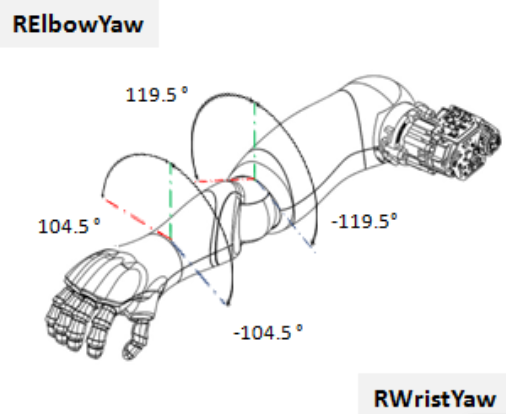
\includegraphics[scale=0.45]{images/RElbowandWrist.png}
        \caption{Right Elbow and Wrist Joint \cite{PepperJoints}}
        \label{fig: Right Elbow and Wrist joint}
    \end{minipage}
\end{figure}

The joint limits for the RElbowRoll is shown in the table \ref{tab:right_arm_joint_limits}.
\begin{longtable}[c]{|l|l|l|l|} 
    \caption{Right arm joint limits. \cite{PepperJoints}} \label{tab:right_arm_joint_limits}\\
    \hline
    \rowcolor{gray!30}
    \textbf{RElbowYaw (°)} & \textbf{RElbowRoll Min (°)} & \textbf{RElbowRoll Max (°)} \\ \hline
    \endhead % header for subsequent pages
    
    -119.5 & 0.5 & 83.0 \\ \hline
    -99.5 & 0.5 & 89.5 \\ \hline
    0.0 & 0.5 & 89.5 \\ \hline
    60.0 & 0.5 & 78.0 \\ \hline
    119.5 & 0.5 & 78.0 \\ \hline

\end{longtable}

\subsection{Hand Actuator Test}
\subsubsection*{Left Hand}
The left hand of the pepper robot articulates a grasp opening and closing. To test the hand, the \texttt{LeftHand} joint is moved 
from the home position to the minimum position and then to the maximum position. Then back to its mid-range position. The terminal output 
will show the result of the test.

The rostopic \texttt{/pepper\_dcm/LeftHand\_controller/follow\_joint\_trajectory} is
used to move the left-hand joint.

The range of the left-hand joint is range from \texttt{0.0 to 1.0}. Where \texttt{0.0} denotes the hand is fully \texttt{closed} and \texttt{1.0} denotes the hand is fully \texttt{open}.

\subsubsection*{Right Hand}

The right hand of the pepper robot articulates a grasp opening and closing. To test the hand, the \texttt{RightHand} joint is moved
from the home position to the minimum position and then to the maximum position. Then back to its mid-range position. The terminal output
will show the result of the test.

The rostopic \texttt{/pepper\_dcm/RightHand\_controller/follow\_joint\_trajectory} moves the right hand joint. The range of the 
right-hand joint is range from \texttt{0.0 to 1.0}. Where \texttt{0.0} denotes the hand is fully \texttt{closed} and \texttt{1.0} denotes 
the hand is fully \texttt{open}.

\subsection{Leg Actuator Test}

The leg of the pepper robot is articulated using three joints:\texttt{HipRoll},\texttt{HipPitch}, and \texttt{KneePitch}. 
These joints are tested sequentially in the listed order to ensure proper functionality and range of motion. The testing 
involves moving each joint through a specific sequence of positions to verify the joint's operational range and functionality 
as follows:\\
$ \texttt{Home pos} \rightarrow \texttt{Minimum pos} \rightarrow \texttt{Maximum pos} \rightarrow \texttt{Mid-range pos} \rightarrow \texttt{Home pos}$.

The rostopic \texttt{/pepper\_dcm/Pelvis\_controller/follow\_joint\_trajectory} moves the leg joint.

Table \ref{tab:leg_joint_range} shows the range of the leg joint.

\begin{longtable}[c]{|l|l|l|l|l|l|} 
    \caption{Leg joint range. \cite{PepperJoints}} \label{tab:leg_joint_range}\\
    \hline
    \rowcolor{gray!30}
    \textbf{Joint} & \textbf{Min (°)} & \textbf{Max (°)} & \textbf{Min (rad)} & \textbf{Max (rad)}  & \textbf{Home (rad)} \\ \hline
    \endhead % header for subsequent pages
    
    \texttt{HipRoll} & -29.5 & 29.5 & -0.5149 & 0.5149 &  -0.00766  \\ \hline
    \texttt{HipPitch} & -59.5 & 59.5 & -1.0385 & 1.0385 & -0.0107   \\ \hline
    \texttt{KneePitch} & -29.5 & 29.5 & -0.5149 & 0.5149 & 0.03221  \\ \hline
    
\end{longtable}

\begin{figure}[!hbpt]
    \centering
    \begin{minipage}{0.45\textwidth}
        \centering
        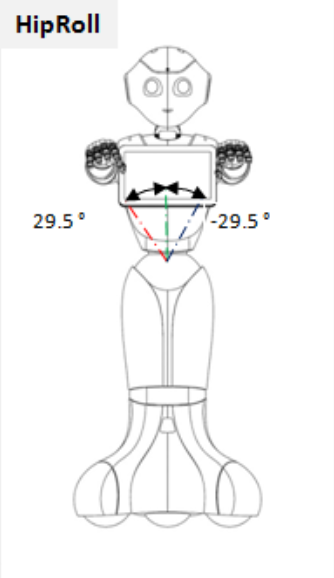
\includegraphics[scale=0.45]{images/HipRoll.png}
        \caption{Hip Roll Joint \cite{PepperJoints}}
        \label{fig: Hip Roll joint}
    \end{minipage}\hfill
    \begin{minipage}{0.45\textwidth}
        \centering
        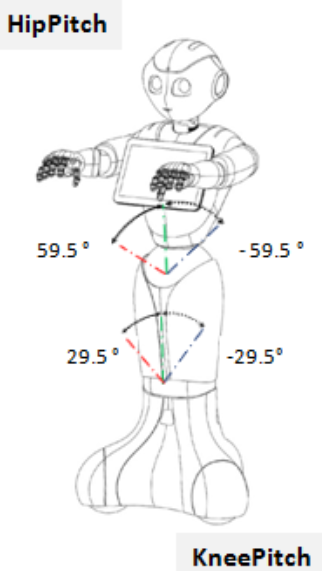
\includegraphics[scale=0.45]{images/HipPitchandKneePitch.png}
        \caption{Hip Pitch Joint and Knee Pitch Joint \cite{PepperJoints}}
        \label{fig: Hip Pitch joint}
    \end{minipage}
\end{figure}

\newpage

\subsection{Wheels Actuator Test}
The pepper robot is equipped with three omnidirectional wheels as shown in Figure \ref{fig: Pepper Wheels}. 
The wheels are tested by moving the robot in a straight line 1 meter forward, and 1 meter backward. Then 
the robot is rotated 90 degrees to the left and 90 degrees to the right. The terminal output will show 
the result of the test.

\begin{figure}[!hbpt]
\centering
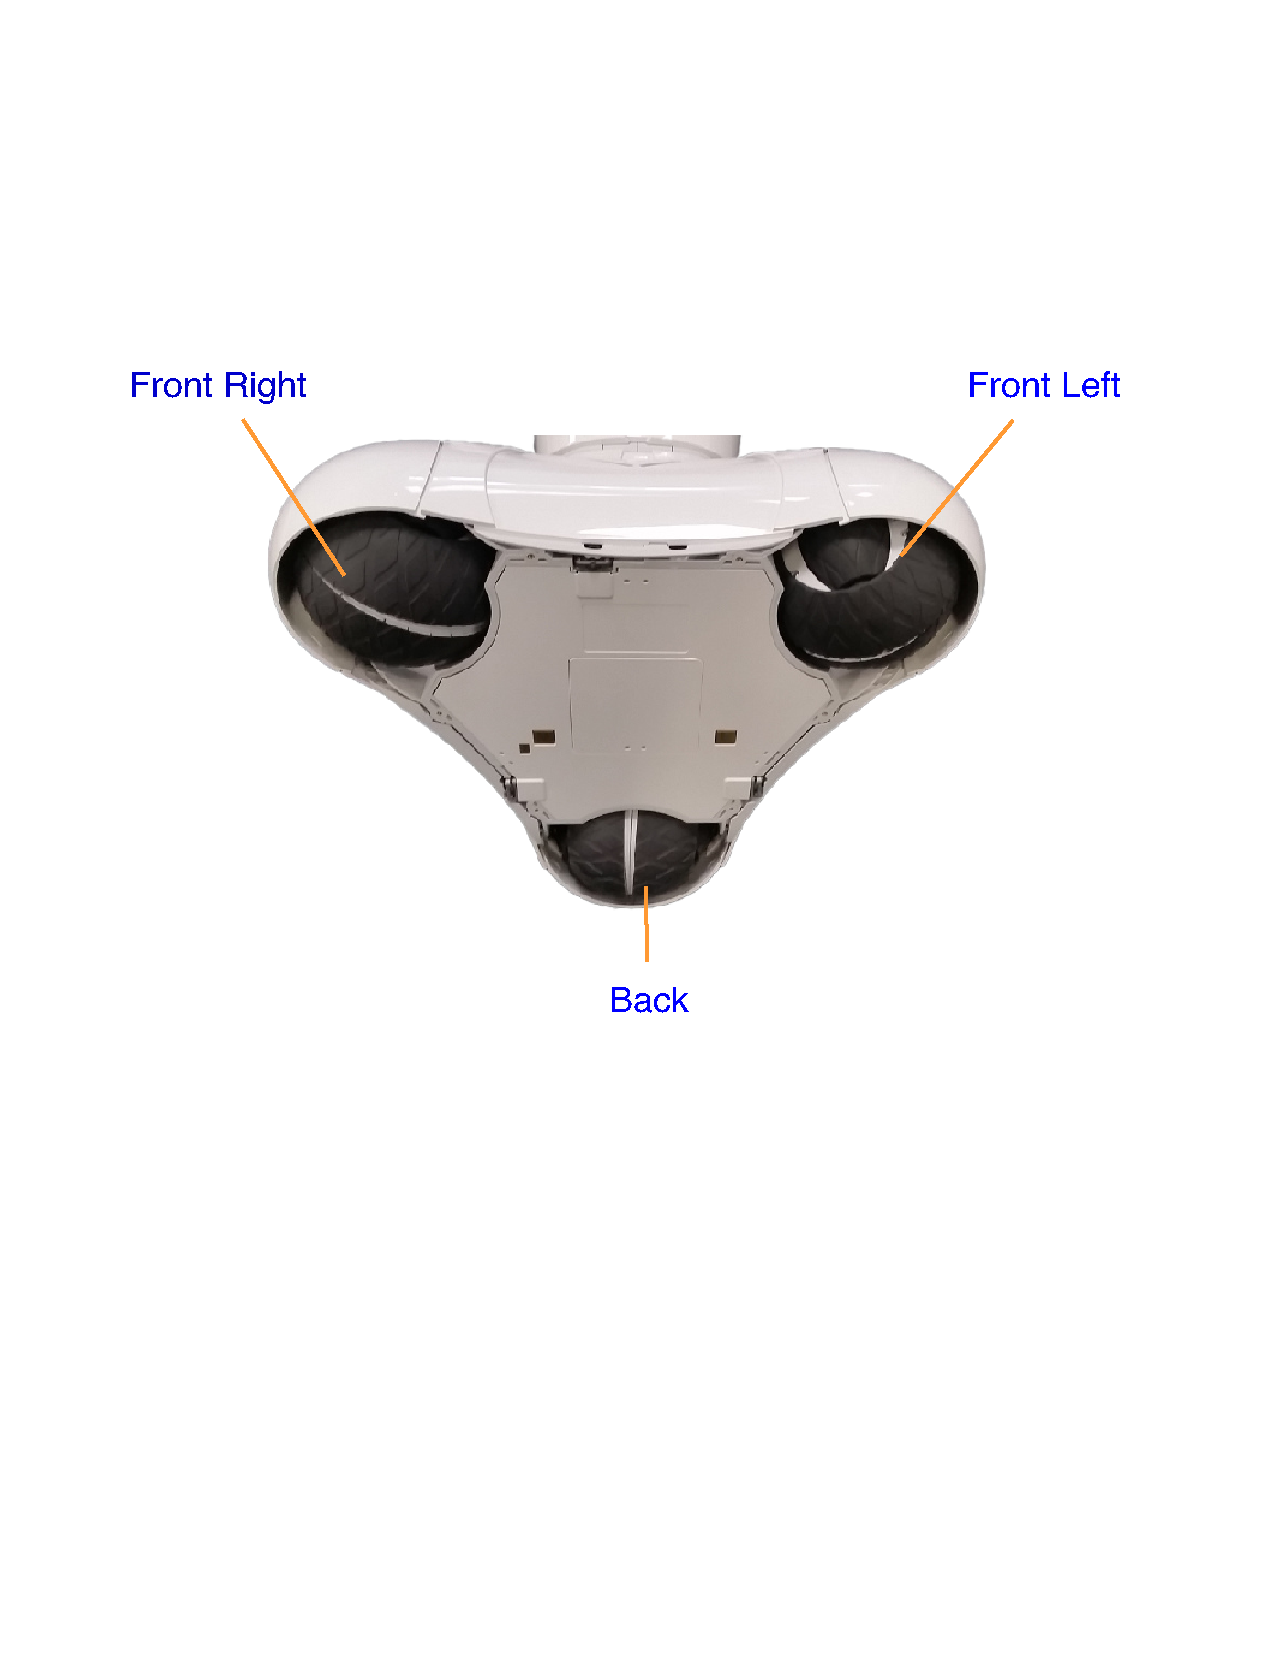
\includegraphics[scale=0.55]{images/Pepper_wheels.pdf}
\caption{Pepper Wheels}
\label{fig: Pepper Wheels}
\end{figure}

\begingroup
\tcbset{%
noteshift/.store in=\mynote@shift,
noteshift=0.8cm
}
\begin{tcolorbox}[nobeforeafter,
enhanced,
sharp corners,
toprule=1pt,
bottomrule=1pt,
leftrule=0pt,
rightrule=0pt,
colback=yellow!20,
left skip=\mynote@shift,
right skip=\mynote@shift,
overlay={\node[left] (mynotenode) at ([xshift=-\mynote@shift]frame.west) {\textbf{\textcolor{greenyellow}{Note:}}} ;},]
Before running the wheels, first move the robot out of the charging dock also close the power hatch 
before launching the actuator test. Furthermore, the user must ensure that the robot is in a safe 
environment to avoid collision with objects. 
\end{tcolorbox}
\endgroup

For testing the wheels, the rostopic \texttt{/cmd\_vel} for the robot and \texttt{/pepper/cmd\_vel} for the simulator is 
used to move the robot. The robot moves in the x-axis direction to move forward and backward given the linear velocity 
and time duration. In addition, the robot rotates in the z-axis direction to rotate counterclockwise and clockwise given
the angular velocity and time duration.


\newpage
\bibliographystyle{unsrt}
%================================================================
\bibliography{cognitive_systems.bib}                                     % REPLACE with correct filename
\addcontentsline{toc}{section}{References}

%------------------------------------------------------------------------------------

\newpage

\section*{Principal Contributors}
%=============================================================
\label{contributors}
\addcontentsline{toc}{section}{Principal Contributors}
The main authors of this deliverable are as follows (in alphabetical order).
\blank
~
\blank
Yohannes Haile, CMU-Africa\\ 
David Vernon, CMU-Africa\\

\pagebreak
\section*{Document History}
%================================================================
\addcontentsline{toc}{section}{Document History}
\label{document_history}

\begin{description}

\item [Version 1.0]~\\
First draft. \\
Yohannes Haile. \\ % REPLACE with the correct name
25 March 2024. % REPLACE with the correct date

\item [Version 1.1]~\\
Changed the title from Source Code \textrightarrow{} File Organization.\\
Yohannes Haile.  \\
30 May 2025.  
    

\end{description}
\end{document}